% Defence deck (~12--15 minutes). Build: pdflatex main.tex (twice) from this folder.
\documentclass[aspectratio=169,11pt,english]{beamer}
\usepackage[T1]{fontenc}
\usepackage{lmodern}
\usepackage{graphicx}
\usepackage{hyperref}
\usepackage{amsmath,amssymb}
\usepackage{babel}

\graphicspath{{assets/}{../outputs/}{../thesis/design/figures/}}

\usetheme{Madrid}
\usecolortheme{seagull}
\setbeamertemplate{navigation symbols}{}

\title[NISQ FRQI]{NISQ-oriented structural optimization of FRQI state preparation for quantum edge detection}
\subtitle{Quantum Computing Master thesis defence}
\author{Alexandru Mitrofan}
\institute{Politehnica University of Timișoara}
\date{June 2026}

\begin{document}

\begin{frame}
  \titlepage
  \note{Introduce yourself; state that the work is simulator-based FRQI + QHED with a controlled comparison of MCX synthesis modes.}
\end{frame}

\begin{frame}{Problem}
  \begin{itemize}
    \item Quantum image pipelines (here: FRQI encoding + QHED) must fit NISQ budgets: depth, CX count, measurement bias.
    \item Multi-controlled address logic dominates FRQI preparation; Qiskit offers different \texttt{MCXGate} synthesis modes (\texttt{noancilla} vs \texttt{v-chain}).
    \item \textbf{Question:} Does switching preparation structure improve \emph{both} resources and application-style scores under matched noise?
  \end{itemize}
  \note{Emphasize this is an engineering trade-off study, not a new edge operator.}
\end{frame}

\begin{frame}{Pipeline (fixed downstream)}
  \begin{itemize}
    \item \textbf{FRQI:} intensities as $R_y$ angles on a color qubit indexed by an address register ($m=2\log_2 N$ qubits).
    \item \textbf{QHED:} FWHT-style stage + classical Sobel scoring on decoded rasters (from \texttt{src/qhed.py}).
    \item \textbf{Compared:} \texttt{MCXGate} \texttt{noancilla} (naive) vs \texttt{v-chain} ancilla pattern; same logical state, same QHED code path.
  \end{itemize}
  \note{Stress that QHED is held constant so differences isolate preparation. Qiskit names: naive maps to noancilla decomposition; v-chain is the ancilla ladder synthesis.}
\end{frame}

\begin{frame}{Where it lives in the repo}
  \begin{itemize}
    \item \textbf{Encoding / QHED / metrics:} \texttt{src/frqi.py}, \texttt{src/qhed.py}, \texttt{src/metrics.py}
    \item \textbf{Structural (naive vs v-chain) circuits:} \texttt{src/improved.py} + driver \texttt{scripts/frqi\_structural\_resources.py}
    \item \textbf{Noise + edges + readout studies:} \texttt{scripts/noisy\_frqi\_sweep.py}, \texttt{scripts/noisy\_recon\_qhed\_edge\_metrics.py}, \texttt{scripts/readout\_mitigation\_shot\_sweep.py}
    \item \textbf{Repro bundle $\rightarrow$ thesis tables:} \texttt{scripts/build\_results\_tables.py} (see thesis Appendix~B).
  \end{itemize}
  \note{Supervisor feedback: tie claims to concrete modules so examiners see the implementation is inspectable.}
\end{frame}

\begin{frame}{Naive vs v-chain (toy view)}
  \begin{center}
    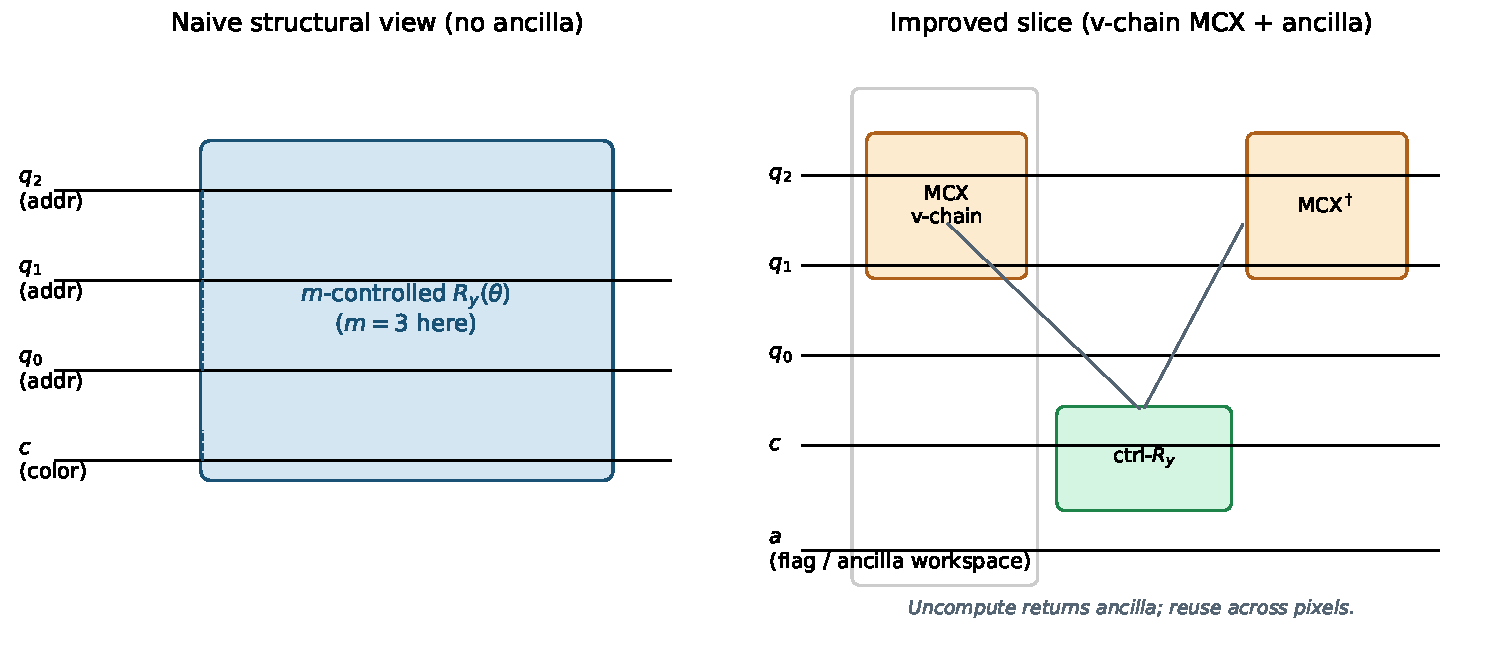
\includegraphics[width=0.88\linewidth,height=0.52\textheight,keepaspectratio]{toy_naive_vs_vchain.pdf}
  \end{center}
  \vspace{-0.35cm}
  {\footnotesize Repository figure: \texttt{thesis/design/figures/} (script \texttt{toy\_and\_block\_level\_diagrams.py}).}
  \note{Left: conceptual single box; right: ancilla ladder + uncompute pattern repeated per pixel in full FRQI.}
\end{frame}

\begin{frame}{Sequential preparation (block view)}
  \begin{center}
    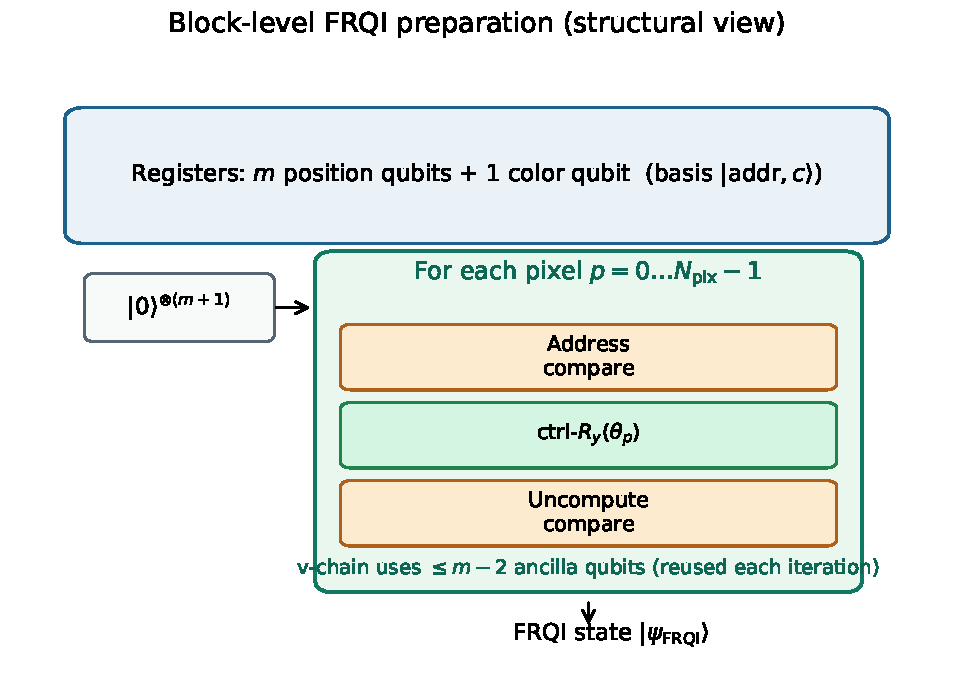
\includegraphics[width=0.85\linewidth,height=0.52\textheight,keepaspectratio]{block_frqi_prep.pdf}
  \end{center}
  \note{Walk through init H on addresses, loop compare--rotate--uncompute, transpile to \{cx,rz,sx\}.}
\end{frame}

\begin{frame}{Minimal transpiled MCX stub}
  \begin{center}
    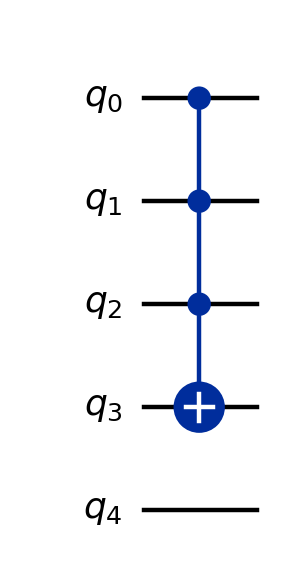
\includegraphics[width=0.88\linewidth,height=0.48\textheight,keepaspectratio]{stub_mcx_vchain.png}
  \end{center}
  {\footnotesize Qiskit transpile preview (\texttt{scripts/qiskit\_stub\_draw.py}).}
  \note{Concrete reminder that ``MCX mode'' is not abstract---it becomes many CX layers after transpilation.}
\end{frame}

\begin{frame}{What we measure}
  \begin{itemize}
    \item \textbf{Resources:} qubits, depth, CX after transpilation (structural study at optimization level~3).
    \item \textbf{Noise:} depolarizing density-matrix sweeps; PSNR, SSIM, fidelity (frozen bundles at optimization level~0).
    \item \textbf{Edges:} QHED vs Sobel SSIM on noisy reconstructions (paired naive vs v-chain rows).
    \item \textbf{Readout:} $2\times2$ confusion matrix inversion slice on $4\times4$ (proof of concept).
  \end{itemize}
  \note{Mention manifests in outputs/ and thesis/results\_configuration.md for reproducibility.}
\end{frame}

\begin{frame}{Structural resources vs image size}
  \begin{columns}[T,onlytextwidth]
    \begin{column}{0.49\linewidth}
      \centering
      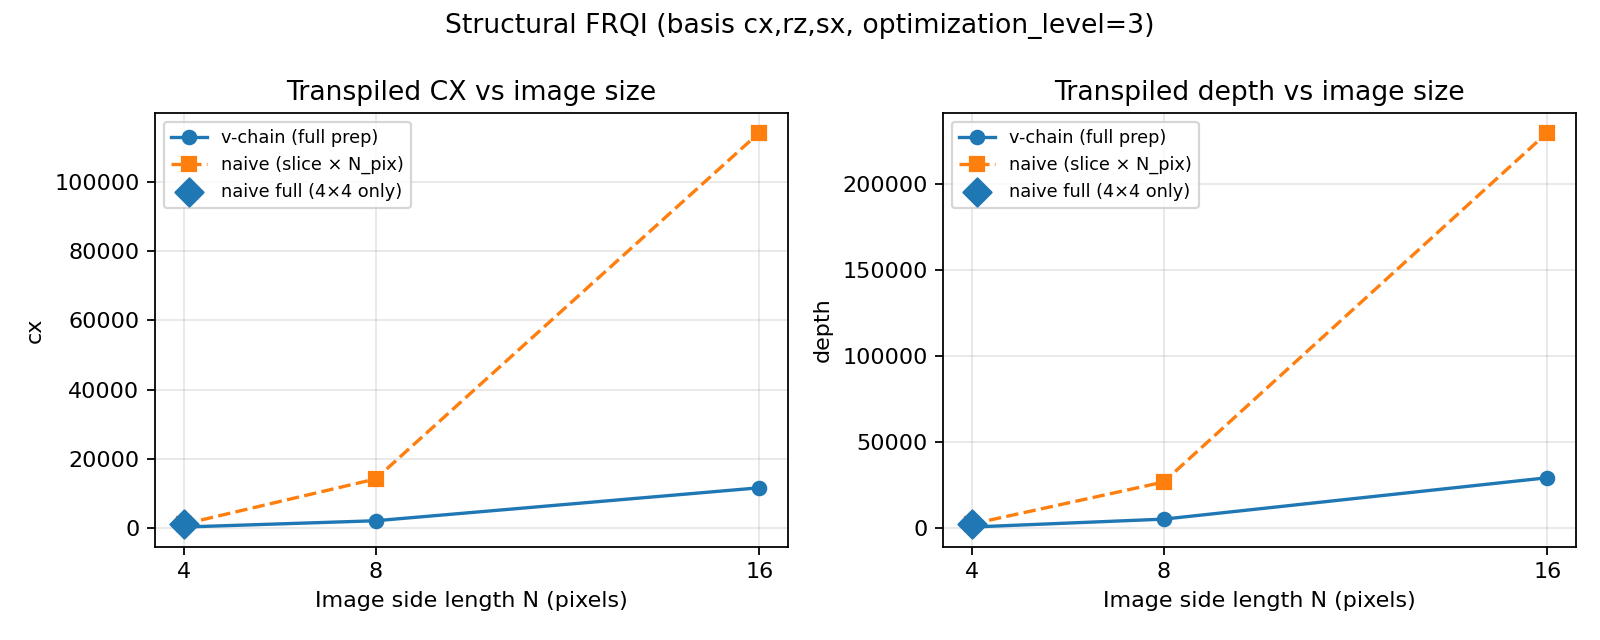
\includegraphics[width=\linewidth,height=0.30\textheight,keepaspectratio]{fig_cx_vs_image_size.png}\\[-0.15em]
      {\scriptsize Transpiled CX (\texttt{optimization\_level}~3)}
    \end{column}
    \begin{column}{0.49\linewidth}
      \centering
      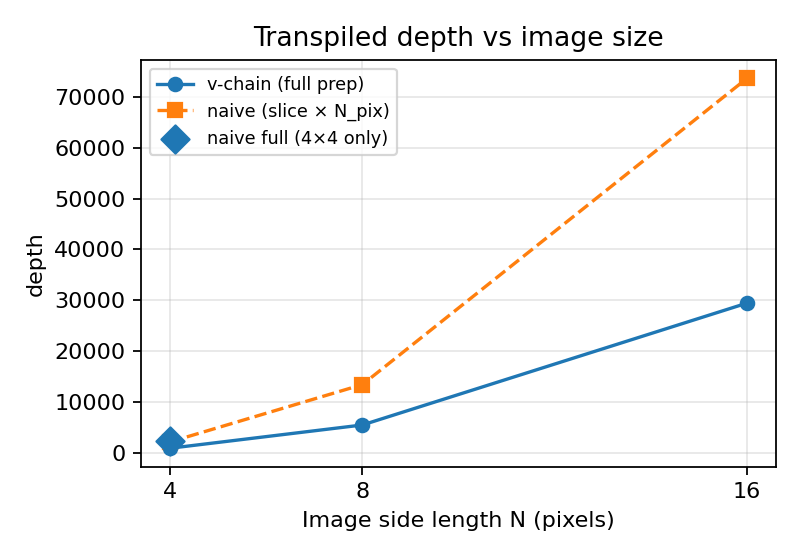
\includegraphics[width=\linewidth,height=0.30\textheight,keepaspectratio]{fig_depth_vs_image_size.png}\\[-0.15em]
      {\scriptsize Transpiled depth}
    \end{column}
  \end{columns}
  \note{Headline: at $16\times16$, v-chain $\approx$11.6k CX vs scaled naive $\approx$114k CX (thesis Results). V-chain uses more qubits but fewer CX layers; DM runtime can still dominate at larger $n$.}
\end{frame}

\begin{frame}{Noisy FRQI ($4\times4$ example)}
  \begin{center}
    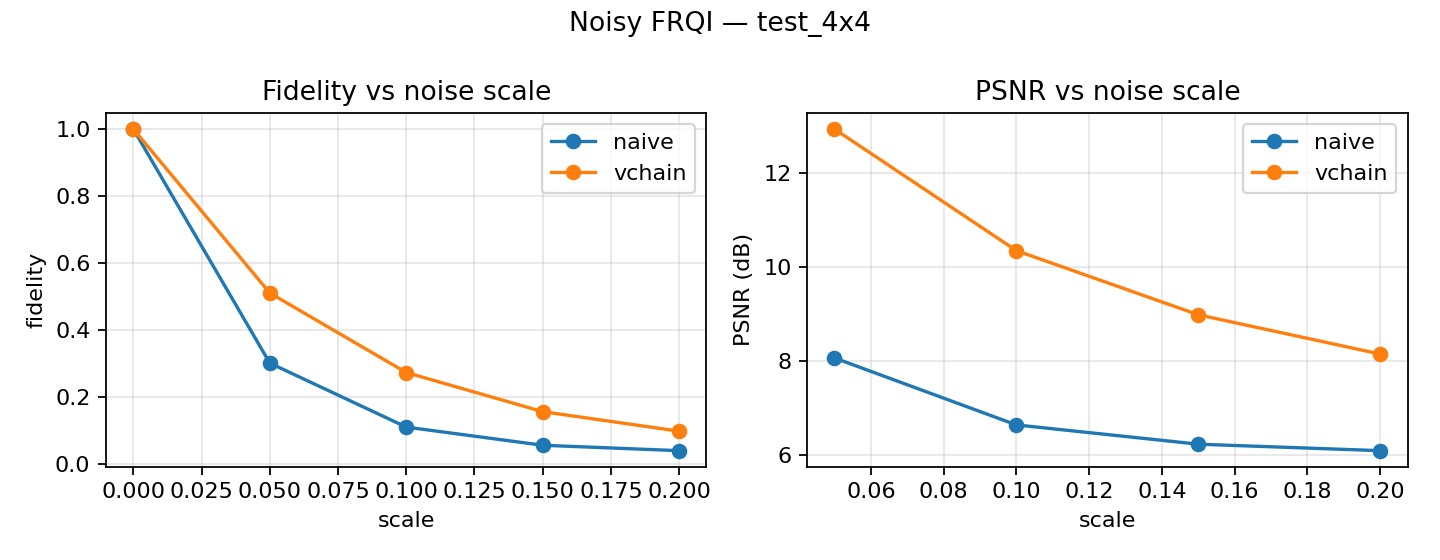
\includegraphics[width=0.88\linewidth]{noisy_frqi_test_4x4_curves.png}
  \end{center}
  \note{Curves can cross---different entanglement patterns accumulate noise differently; do not read only CX.}
\end{frame}

\begin{frame}{Readout mitigation (synthetic)}
  \begin{center}
    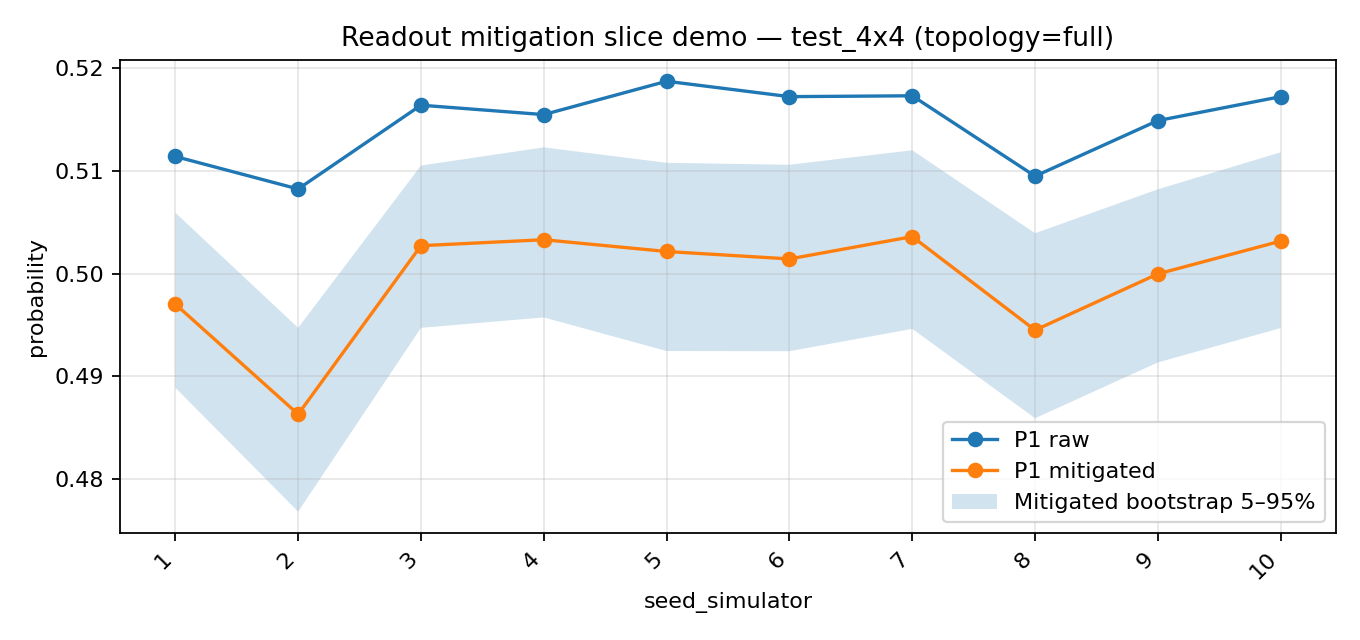
\includegraphics[width=0.72\linewidth]{readout_mitigation_shot_sweep.png}
  \end{center}
  \note{Shows systematic shift in inferred $p_1$ across seeds on a toy confusion model; separate from depolarizing DM study.}
\end{frame}

\begin{frame}{Main takeaway}
  \begin{itemize}
    \item V-chain can \textbf{substantially reduce} transpiled CX/depth for the same FRQI state at larger $N$.
    \item Under the thesis noise grid, \textbf{edge SSIM does not} show a significant naive$\rightarrow$v-chain win (exploratory Wilcoxon $p\approx0.078$ on eight paired noise cells).
    \item \textbf{Lesson:} report resources \emph{and} application metrics; gate-count reductions are not automatic image wins on NISQ-style models.
  \end{itemize}
  \note{Honest limitation: simulator only; 16$\times$16 v-chain DM often skipped; scaled naive extrapolates one slice.}
\end{frame}

\begin{frame}{Limitations \& future work}
  \begin{itemize}
    \item No hardware shots; mock NISQ bundle is optional evidence only.
    \item Tiny images; small statistical $n$; scaled naive baseline extrapolates from one transpiled slice.
    \item Missing v-chain noisy/edge cells at $16\times16$ (density-matrix cost); Wilcoxon uses eight paired cells only.
    \item Future: layout-aware hardware runs, richer mitigation, complete v-chain DM at $16\times16$ if memory allows.
  \end{itemize}
  \note{Align with Conclusions: under-claim relative to the resource win; honest about extrapolation and missing cells.}
\end{frame}

\begin{frame}[c]
  \centering
  \Large Thank you!
  \vspace{0.8em}
\end{frame}

\appendix

\begin{frame}{Backup: reproduction order (thesis App.~B)}
  \small
  \begin{enumerate}
    \item \texttt{pytest}
    \item \texttt{python scripts/frqi\_qhed\_sobel.py}
    \item \texttt{python scripts/frqi\_structural\_resources.py}
    \item \texttt{python scripts/noisy\_frqi\_sweep.py} (\texttt{--allow-heavy-dm} only if RAM allows)
    \item \texttt{python scripts/noisy\_recon\_qhed\_edge\_metrics.py}
    \item \texttt{python scripts/readout\_mitigation\_shot\_sweep.py}
    \item \texttt{python scripts/build\_results\_tables.py --require-figures}
  \end{enumerate}
\end{frame}

\end{document}
